\documentclass{standalone}
\usepackage{tikz}
\usepackage{ctex,siunitx}
\setCJKmainfont{Noto Serif CJK SC}
\usepackage{tkz-euclide}
\usepackage{amsmath}
\usetikzlibrary{patterns, calc,3d}
\usetikzlibrary {decorations.pathmorphing,decorations.pathreplacing,decorations.shapes}
\begin{document}
\small
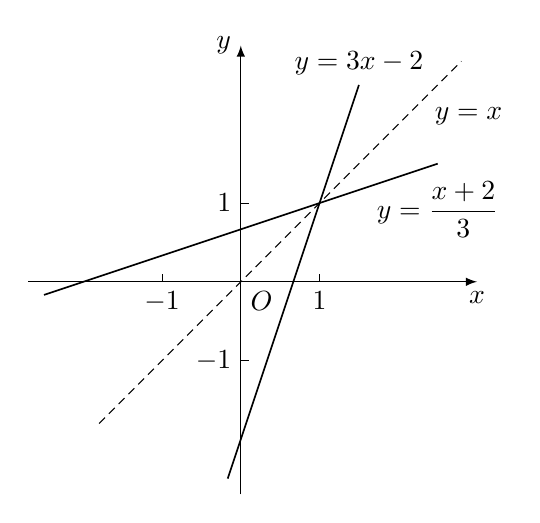
\begin{tikzpicture}[>=latex,scale=1.0]
  \draw[->](-2.7,0)--(3.0,0)node[below]{$x$};
  \draw[->](0,-2.7)--(0,3.0)node[left]{$y$};
  \node at (0,0)[below right]{$O$};
  \draw[densely dashed](-1.8,-1.8)--(2.8,2.8)node[pos=0.9,below right]{$y=x$};
  \draw[semithick](-2.5,-1/6)--(2.5,1.5)node[below=3pt]{$y=\dfrac{x+2}{3}$};
  \draw[semithick](-1/6,-2.5)--(1.5,2.5)node[above]{$y=3x-2$};
  \foreach \x in {1,-1} 
    { 
      \draw[very thin] (\x,0)node[below]{$\x$}--++(0,0.1); 
      \draw[very thin] (0,\x)node[left]{$\x$}--++(0.1,0); 
    }
\end{tikzpicture}
\end{document}